\documentclass[../root]{subfiles}
\graphicspath{{_images/}{../_images/}}


\begin{document}

    \chapter{Status Goods: Experimental evidence from platinum credit cards}

    \begin{shortsummary}
        \begin{itemize}
            \item \authoryear{Bursztyn2018}
            \item \RQ{Does a desire to signal high income or wealth cause consumers to purchase status goods?}
            \item \answer{A series of field experiment with credit card market}
            \item \result{The status aspect of a premium credit card is an important driver of demand for the product, over and above its instrumental benefits.}
        \end{itemize}
    \end{shortsummary}

    \section{Introduction}

    \begin{figure}[h]
        \centering
        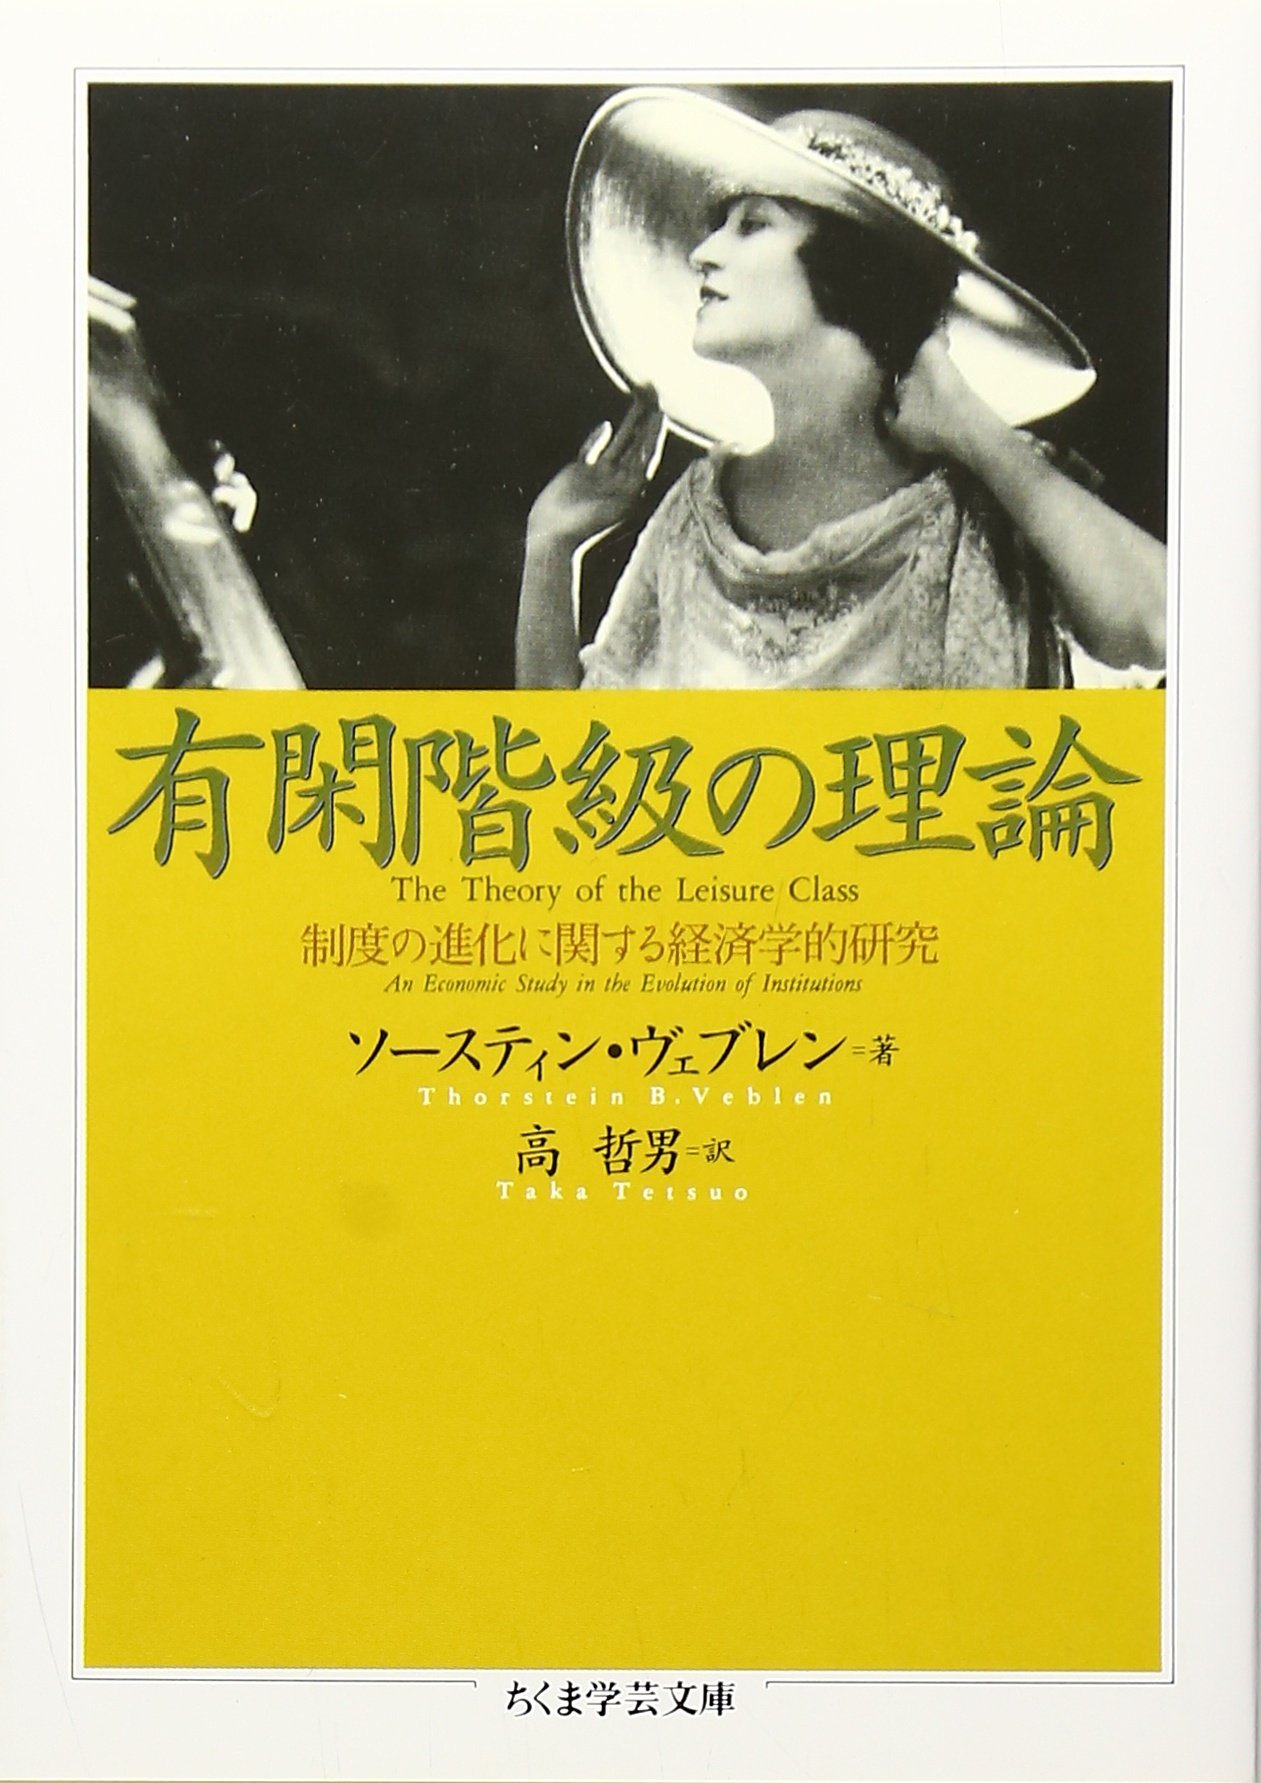
\includegraphics[width = 0.5\linewidth]{0717kato/veblen.jpg}
        \caption{Veblen's Famous Book}
        \label{veblen}
    \end{figure}

    \begin{quote}
        日常生活における冷淡な観察者たちに、自らの金銭的能力を見せつけるために利用しうる唯一の手段は、たえず支払能力を見せつけることである(ソースティン・ヴェブレン「有閑階級の理論」)
    \end{quote}

    \begin{itemize}
        \item A fundamental economic behavior - consumption - may be shaped by social image concerns.
        \begin{itemize}
            \item A desire to signal high income or wealth cause consumers to purchase status goods (conspicuous consumption 顕示的消費).
        \end{itemize}
        \item With observational data, it is difficult to fully separate unobserved consumption utility from a desire to signal high income.
        \item Self-image or identity and the demand for status could be deeply connected, and it remains an open question whether self- and social image are substitutes or complements.
        \item This paper (i) provides field-experimental evidence of the existence of status goods; (ii) test fot the associated positional externalities; and (iii) shed light on how self-image interacts with social image in explaining the demand for status.
        \begin{itemize}
            \item Design three related experiments and one observational study with a large bank in Indonesia to market the bank's widely recognized platinum credit card.
        \end{itemize} 
    \end{itemize}

    \section{Background of Credit Cards}

    \begin{figure}[h]
        \centering
        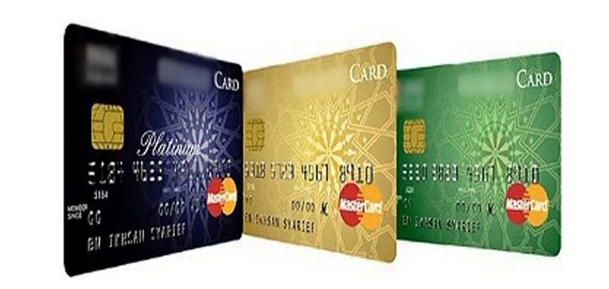
\includegraphics[width = 0.7\linewidth]{0717kato/creca.PNG}
        \caption{Credit Cards}
        \label{creca}
    \end{figure}
    

    \begin{itemize}
        \item The bank has approximately 200,000 credit card customers and offers its credit card product in three tires: classic, gold, and platinum.
        \begin{itemize}
            \item The three tires are vertically differentiated based on income: The platinum card has the highest income eligibility criterion, and the classic card with the lowest income requirement.
            \item Only 10\% of active credit card customers at the bank qualify fot a platinum card, 72\% of card customers have a gold card, and the remaining 18\% qualify only for the classic card.
            \item The bottom quartile of the customer population is close to the median income of urban Indonesia, while the median credit card customer is in the top 15\% of urban incomes in Indonesia.
            \item The platinum card differs from the two lower-tier cards in both color and design: it is dark purple and has the word \textit{Platinum} printed in large cursive letters across the front of the card.
        \end{itemize}
        \item A necessary condition for status signaling is public recognition of the platinum card
        \begin{itemize}
            \item Conduct surveys outside malls in the greater Jakarta area.
            \item First survey (N = 113): 93 out of 113 ranked the cards correctly in terms of their income requirements.
            \item Second survey (N = 500): 59\% of respondents recognized the platinum card as having a higher income criterion. Restricting those who have a credit card or report having seen a platinum credit card before, this share increases to 71\%
            \item The platinum card can serve as a means to signal higher income, especially to an audience more familiar with credit cards.
        \end{itemize}
    \end{itemize}

    \section{Experiment 1: Demand For the Platinum Card versus Its Instrumental Benefits}

    \begin{itemize}
        \item Goal: to test whether part of the demand for the platinum card is unrelated to its instrumental features
        \item Sample: 1,260 customers randomly drawn from the set of current gold card holders with relatively high income. These were customers to whom the bank was willing to offer an upgrade to the platinum card, even though they may not have normally qualified for it.
        \item Treatment:
        \begin{enumerate}
            \item \textit{Platinum upgrade treatment}: customers were offered an upgrade the the bank's regular platinum card.
            \item \textit{Benefits upgrade treatment}: customers were offered the same services as the platinum card, but as an add-on their current gold card.
            \item \textit{Platinum upgrade merit treatment}: Instead of being told they were randomly chosen, they were told, ``As one of our top customers, you have been chosen to receive an upgrade to our platinum card.''
        \end{enumerate}
        \item Implementation: The experiment was conducted over the course of one week. Each day, four callers made phone calls to a randomly assigned list of credit card customers from the sample. Each client received the offer only once, but up to three call attempts were made if a client could not be reached or was busy at the time of a previous attempt. However, no additional calls were made once any part of the offer had been revealed to a respondent. The callers were able to reach 835 out of 1260 clients, 
    \end{itemize}

    \begin{figure}[h]
        \centering
        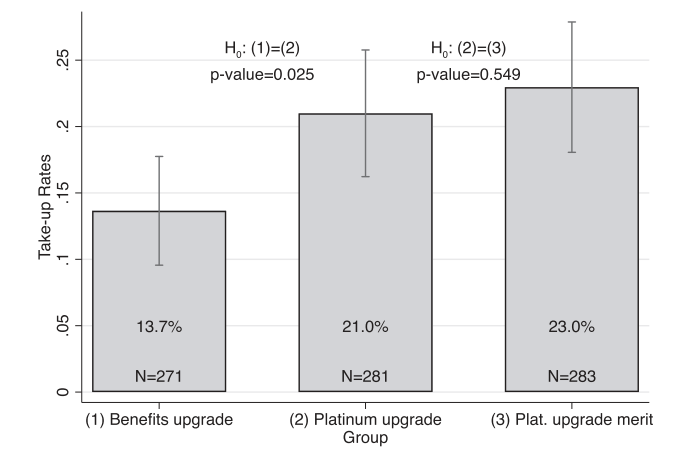
\includegraphics[width = 0.8\linewidth]{0717kato/result_exp1.PNG}
        \caption{Result of Experiment 1}
        \label{result1}
    \end{figure}

    \begin{itemize}
        \item What we learn from figure \ref{result1}: 
        \begin{itemize}
            \item Strong demand for the physical appearance of the new card the customers receive.
            \item Informing customers they had been randomly chosen to receive the platinum offer was not perceived as off-putting or particularly unnatural.
        \end{itemize}
        \item Other remarks:
        \begin{itemize}
            \item the bank made a second call to customers who had declined the offer when they were first contacted and offered them the same upgrade at a 25\% discount. This increased demand for the benefits upgrade by only 3.7\% points.
            \item One potential confounding is customer suspicion, confusion, or offence. This is not serious because only 1\% of the respondents stated that they had doubts that the quality of the benefits and services would be identical to the platinum card, and None of the respondents reported being offended about not being offered the actual platinum card (follow-up survey).
        \end{itemize}
    \end{itemize}


    \section{Observational Study: Status Signaling in Credit Card Transaction Data}

    \begin{itemize}
        \item Credit card transaction data for customers with active credit cards who opened their accounts between January 2014 and August 2015, and who have gold card with Rp 20 million or Rp 30 million credit limits (the highest credit limit) or platinum card with Rp 40 million and Rp 50 million credit limit (the lowest credit limit).
        \item Using detailed information on the transaction amount, transaction type, and location, they categorize transactions as either visible, online, or retail.
        \begin{itemize}
            \item \textit{visible} transaction: restaurants, cafes, and bars (89\%), in membership clubs (2\%), movie theaters (2\%), and other amusement and recreational services (7\%)
            \item \textit{online} transaction: transactions with internet-related terms, such as ``www,'' ``.com'', or ``e-store,'' in the text description
            \item \textit{retail} transaction: supermarkets, grocery and convenience stores (30\%), department stores (10\%), service stations (7\%), clothing stores (6\%), and at other merchants, such as pharmacies (47\%).
        \end{itemize}
        \item Variation in credit limits as a proxy for income and creditworthiness.
        \begin{itemize}
            \item Main: compare the lowest-income platinum card holders (Rp 40 million credit limit) with the highest-income gold card holders (Rp 30 million credit limit).
            \item Ruling out confounder: compare within the platinum card group (Rp 40 million versus Rp 50 million credit limit) and within the gold card group (Rp 20 million versus Rp 30 million credit limit)
        \end{itemize}
    \end{itemize}

    \begin{figure}[h]
        \centering
        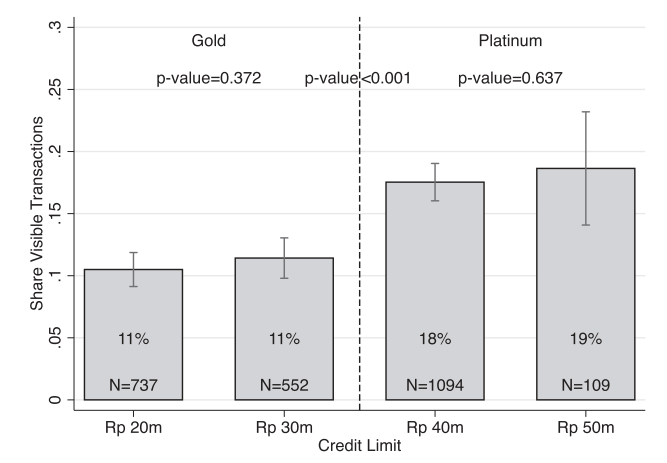
\includegraphics[width = 0.8\linewidth]{0717kato/result_obs.PNG}
        \caption{Share of Visible Transaction}
        \label{result2}
    \end{figure}

    \begin{itemize}
        \item What we learn from the figure \ref{result2}
        \begin{itemize}
            \item Platinum card holders use their card to signal income to their peers in social settings.
            \item The main difference is not simply related to a credit limit increase. 
        \end{itemize}
        \item Other remarks
        \begin{itemize}
            \item There is not significant change in the share of online transactions between the gold card with Rp 30m and the platinum card with Rp 40m, and a significant decrease in the proportion of retail transactions.
        \end{itemize}
        \item Interpretation: A costly signal
        \begin{itemize}
            \item From a retrospective consumption survey, having a platinum card does not make customers more likely to go to restaurants. However, they use different modes of payment for these restaurant expenditures.
            \item This result does not come from price effects since the platinum card does not offer cash back or discounts in restaurants. Instead, 48\% of platinum card customers own other credit cards that do offer cash back rewards.  
            \item Platinum card holders therefore appear willing to pay a cost to show off their card, forgoing cash back from other credit cards.
        \end{itemize}
    \end{itemize}


    \section{Experiment 2: Positional Externality}

    \begin{itemize}
        \item Goal: to show negative positional externality: 
        \begin{itemize}
            \item When individuals with comparatively lower social status gain access to a status good, it diminishes its signaling value and imposes a negative positional externality on the current owners of the status good. This, in turn, should induce the earliest adopters to demand a more exclusive status good
        \end{itemize}
        \item Sample: 180 platinum card customers, who joined under the old income requirement and were unaware of the recent change in the platinum credit card's income eligibility.
        \item Treatment: A costly take-up experiment in which they offered the diamond card, which is the card that the bank was considering the introduction of a new credit card tier above platinum.
        \begin{itemize}
            \item \textit{Control}: The caller explained that the diamond card would have the exact same services, benefits, credit limit, and additional services as the platinum card, but would differ in color and design.
            \item \textit{Positional externality treatment}: Additional information that the bank had recently relaxed the eligibility criteria for the platinum card
        \end{itemize}
    \end{itemize}

    \begin{figure}[h]
        \centering
        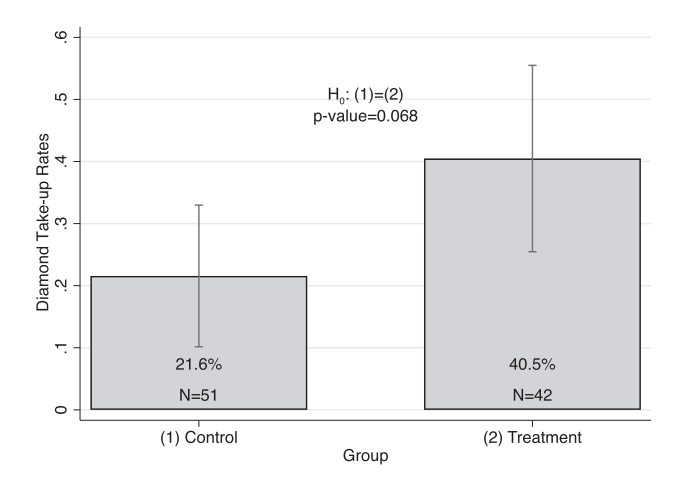
\includegraphics[width = 0.8\linewidth]{0717kato/result_exp2.PNG}
        \caption{Result of Experiment 2}
        \label{result3}
    \end{figure}

    \begin{itemize}
        \item What we learn from figure \ref{result3}
        \begin{itemize}
            \item Demand for the diamond card increases when customers are informed that the platinum card is now available to a wider group of customers.
            \item As lower-status consumers begin adopting the status good, they cause higher-status consumers to demand more exclusive products.
        \end{itemize}
    \end{itemize}


    \section{MTurk Experiment: Self-Image and Status Goods}

    \begin{itemize}
        \item Goal: to test whether high self-esteem, which is an important component of self-image, affects the demand for status goods
        \begin{itemize}
            \item high-income individuals might demand status goods because they derive utility from making consumption choices consistent with their self-image, irrespective of the social visibility of their consumption. 
        \end{itemize}
        \item Sample: 405 individuals who signed up for an incentivized task on the online platform MTurk in August 2016.
        \item Treatment: In the first part of the experiment, participants were randomly assigned to one of two tasks. In the second part of the experiment, all participants were asked to make incentivized MPL choices between gift certificates of different amounts, one for a classic status good (luxury apparel), and the other for a control product (non-luxury apparel).
        \begin{itemize}
            \item \textit{treatment}: to write a paragraph about a recent experience or achievement that made them proud (self-affirmation exercise adapted from the psychology literature)
            \item \textit{control}: to write the title and summarize the story of the last movie you have seen
            \item Participants in the treatment group scored 1.22 points higher on the self-esteem Rosenberg measure than participants in the control group (statistically significant at the 10\% level).
        \end{itemize}
    \end{itemize}

    \begin{figure}[h]
        \centering
        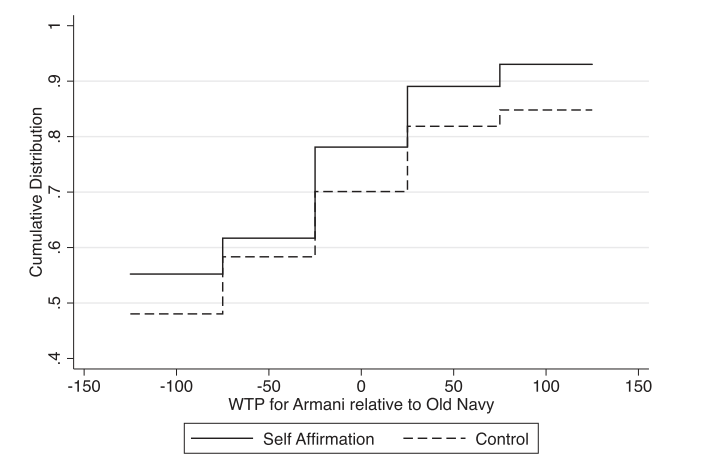
\includegraphics[width = 0.8\linewidth]{0717kato/result_exp3.PNG}
        \caption{Self- and Social Image}
        \label{result4}
    \end{figure}

    \begin{itemize}
        \item What we learn from figure \ref{result4}
        \begin{itemize}
            \item The self-affirmation treatment has a negative effect on the willingness to pay for the Armani gift card.
            \item Higher self-image reduces individuals' desire for social image, and thus their demand for status goods. That is, self- and social image are substitutes.
        \end{itemize}
    \end{itemize}


    \section{Conclusions}

    \begin{quote}
        we show that the status aspect of a premium credit card - due to its potential to signal income - is an important driver of demand for the product, over and above its instrumental benefits. Our experiments also identify a positional externality associated with the consumption of these status goods, thus con- firming a key aspect of theories of status goods. We also provide suggestive evidence that higher self-esteem causally reduces demand for status goods, implying that self- and social image are substitutes (\citealp[p.1593]{Bursztyn2018}).
    \end{quote}



    \biblio

\end{document}